\section{Theorie}
\label{sec:Theorie}

Aufgrund der Quantisierung von sowohl Licht, als auch der Elektronen-Energieniveaus, tritt der Photoeffekt
erst ab einer gewissen Wellenlänge von Licht auf. Dies liegt an der Frequenz-Abhängigkeit
\begin{equation}
    E=\hbar \omega
    \label{eqn:photon}
\end{equation}
\noindent der Energie der Photonen. Dazu werden Elektronen erst von ihren Atomen gelöst, wenn die Energie $E_\gamma > \phi$
ist, wobei $\phi$ die Austrittsarbeit für das Elektron ist. Als Konsequenz sorgt nicht die Intensität des Lichts dafür,
dass Elektronen gelöst werden, sondern nur die Energie der Photonen. Die Intensität ist hier nur ein Maß für die Menge
an Elektronen, die gelöst werden, da es mehr Photonen gibt, die diese Lösen können. \\
Zur Bestimmung der kinetischen Energie der gelösten Elektronen wird dann die Gegenfeldmethode verwendet. Für die Energie 
der Elektronen lässt sich daraus
\begin{align}
    E_{kin}=&E_{el}\\
    \iff \frac{1}{2}mv^2=eU
    \label{eqn:ekin}
\end{align}
\noindent schließen, wenn die Teilchen an der Anode stehen bleiben würden bzw. nicht mehr ankommen.
Für die Energie der Photonen lässt sich dann schließen, dass sie
\begin{equation}
    \hbar \omega=\phi+eU
    \label{eqn:hquer}
\end{equation}
\noindent betragen muss. \\
\noindent Die Wahrscheinlichkeit, dass Elektronen eine gewisse Energie bestitzen wird durch eine Fermi-Dirac Verteilung beschrieben.
\begin{figure}[H]
    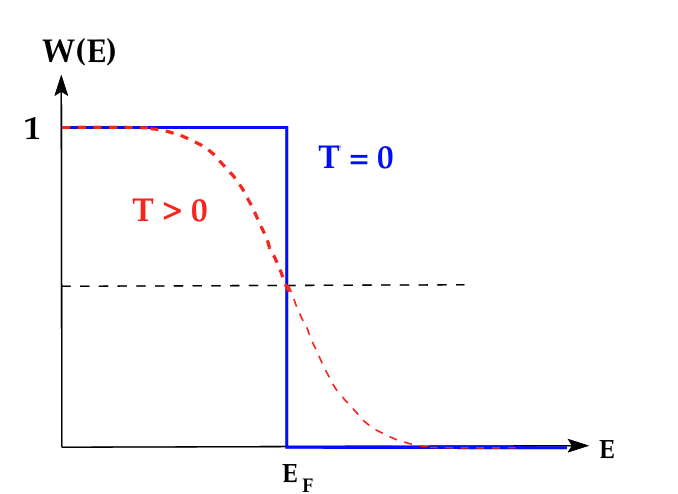
\includegraphics{Bilder/fermi-dirac.png}
    \centering
    \caption{Darstellung der Fermi-Dirac Verteilung}
    \label{fig:fermidirac}
\end{figure}
\noindent Dadurch steigt der gemessene Photostrom tatsächlich nicht linear mit zunehmender Energie, sonder annähernd quadratisch
um die $0$ herum.
\cite{sample}
